\begin{figure}[!ht]
  \centering
  \begin{subfigure}[b]{0.47\linewidth}
    
\includegraphics[width=\linewidth]{images/dap}
    \caption{}
    \label{fig:dap}
  \end{subfigure}
%
  \begin{subfigure}[b]{0.47\linewidth}
    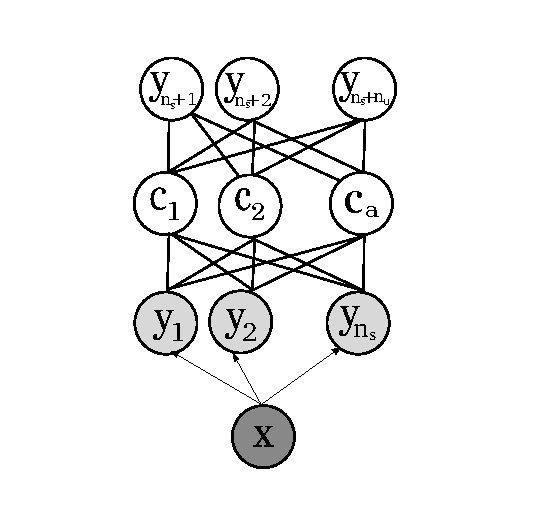
\includegraphics[width=\linewidth]{images/iap}
    \caption{}
% \caption{Points colored according to their ground truth labels}
    \label{fig:iap}
  \end{subfigure}
  \caption[مدل گرافی پیش‌بینی ویژگی مستقیم و غیرمستقیم]{
  مدل گرافی پیش‌بینی ویژگی مستقیم (آ) و غیر مستقیم (ب). رئوس با سایه‌ی روشن رئوسی هستند که در زمان آموزش رویت شده هستند و رئوس با سایه‌ی تیره همواره رویت شده‌اند. رئوس بدون سایه مربوط به متغیرهایی است که باید استنتاج در مورد آن‌ها انجام شود. یال‌های ضخیم‌تر روابط ثابت را نشان می‌دهند که جزو داده‌های آموزش هستند و یال‌های نازک‌تر روابطی را که باید کشف شوند. $x$ یک تصویر است، متغیرهای دودویی
  $y_1, \ldots y_{n_s}$
  تعلق یا عدم تعلق تصویر به دسته‌های دیده شده و بصورت مشابه 
  $y_{n_s +1}, \ldots y_{n_s+n_u}$
  تعلق یا عدم تعلق به دسته‌های دیده نشده را نشان می‌دهند. 
  $c_1, \ldots, c_a$
  ویژگی‌های توصیف‌کننده دسته‌ها هستند.
\textbf{آ)}
در مدل پیش‌بینی ویژگی مستقیم رابطه میان برچسب‌ها و ویژگی‌ها ثابت فرض می‌شود و هدف استنتاج ویژگی از روی تصاویر است. بعد از آن با استفاده از رابطه از پیش تعیین شده برچسب‌ها با ویژگی‌ها، برچسب تعیین می‌شود. 
\textbf{ب)}
در مدل پیش‌بینی ویژگی غیر مستقیم، یک دسته‌بند چنددسته‌ای روی دسته‌های آموزش یادگرفته می‌شود و با توجه به وقوع یا عدم وقوع هر یک از ویژگی‌ها در این دسته‌ها رابطه‌ی ثابتی میان دسته‌های دیده شده 
$y_1, \ldots y_{n_s}$
و ویژگی‌ها فرض می‌شود. هم‌چنین رابطه ویژگی‌ها با دسته‌های دیده نشده 
$y_{n_s +1}, \ldots y_{n_s+n_u}$
رابطه امضا بودن است و دانسته فرض می‌شود \cite{lampert09}.
  }
  \label{fig:diap}
\end{figure}
